\documentclass[article,latterpaper]{IEEEtran}
\usepackage[utf8]{inputenc}
\usepackage{float}
\usepackage[spanish]{babel}
\usepackage{geometry}
\usepackage{url}
\usepackage{cite}
\usepackage{graphicx}
\usepackage{subfigure}
\usepackage{amssymb}
\usepackage{amsmath}
\usepackage{hyperref}
\usepackage{xurl}
\usepackage{caption}
\usepackage{array}
\usepackage{multirow}
\usepackage{makecell}
\usepackage{comment}
\usepackage{fancyhdr}

\title{Introducción a la Computación Científica de Alto Rendimiento\\Proyecto: Solución de la ecuación de difusión}
\author{
\IEEEauthorblockN{Kevin Steven Cortés Rincón\IEEEauthorrefmark{1}}
\IEEEauthorblockA{\textit{kcortes@unal.edu.co}\\\IEEEauthorrefmark{1}Departamento de ingeniería mecánica y mecatrónica, Universidad Nacional de Colombia, Sede Bogotá}
}
\date{\today}
\begin{document}

\maketitle

\section{Introducción}
El proyecto realizado para el primer módulo del curso \textit{introducción a la computación científica de alto rendimiento} es la implementación del método de volúmenes finitos (FVM por sus siglas en Inglés) para solucionar la ecuación de difusión en un problema de conducción de calor en una placa rectangular en estado estacionario.

Ahora bien, el flujo de trabajo llevado a cabo es:

\begin{itemize}
	\item Discretización a mano de la ecuación de difusión.
	\item Programación de la malla.
	\item Programación de las propiedades físicas y del término fuente.
	\item Programación de las condiciones de frontera.
	\item Programación de la etapa de procesamiento: La solución del sistema de ecuaciones se realizó mediante el método iterativo de Gauss - Seidel.
	\item Programación de la etapa de posprocesamiento: Obtención de las gráficas que muestran los resultados.
\end{itemize}

Cada vez que se obtuvo avances los archivos y casos fueron subidos a un repositorio de GitHub cuyo enlace es: \url{https://github.com/KevinCortesR/Proyecto_ICCAR.git}

\vspace{1.5 cm}

Por otra parte, para comprobar el funcionamiento de los códigos realizados se hizo la implementación de un caso con solución analítica. Una vez comprobados, se solucionó el problema de interés y se analizaron los resultados.

\section{Problema de interés}
Se tiene una placa plana como se muestra a continuación:

\begin{figure}[H]
    \centering
    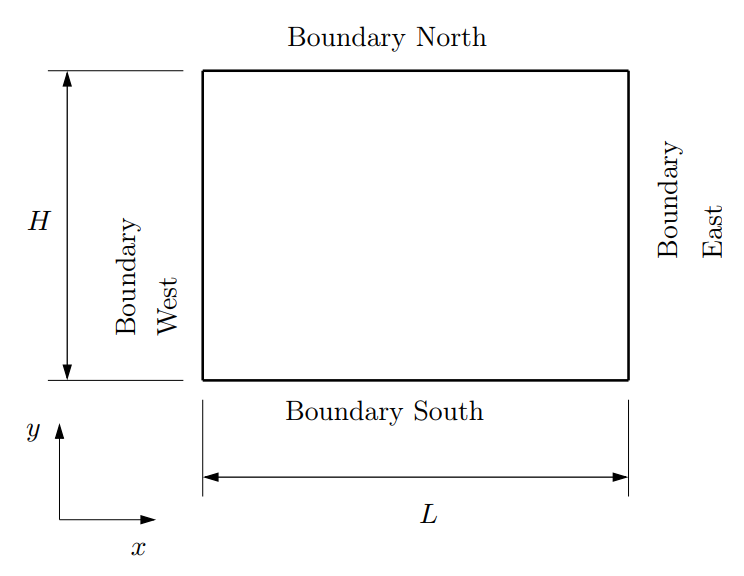
\includegraphics[scale=0.3]{Prob_CFD1.png}
    \caption{ \centering{Geometría de la placa: $L=3$ m y $H=2$ m}}
    \label{Dom_cp}
\end{figure}

Para esta placa se tienen las siguientes condiciones de frontera, conductividad témica y término fuente:

$$
\begin{array}{|cc|}
    \hline \text { Frontera } & \text { Condición } \\
    \hline \text { Norte } & \frac{\partial T}{\partial y}=0 \text { (adiabatica) } \\
    \text { Sur } & T=-5+20\left(\frac{x}{L}\right)^2+20 \sin \left(\frac{4 \pi x}{L}\right) \\
    \text { Oeste } & T=-5^{\circ} \mathrm{C} \\
    \text { Este } & T=15^{\circ} \mathrm{C} \\
    \hline \text { Conduct. } & \kappa=2\left(2.5-\frac{x}{L}\right) \mathrm{W} / \mathrm{m} \cdot{ }^{\circ} \mathrm{C} \\
    \text { Fuente } & B=100 \\
    \hline
\end{array}
$$

La ecuación de difusión que rige el problema es la siguiente:

\begin{equation}
    0 = \frac{\partial}{\partial x} \left( \kappa \frac{\partial T}{\partial x}  \right) +  \frac{\partial}{\partial y} \left( \kappa \frac{\partial T}{\partial y}  \right) +B
    \label{Ec_difusion}      
\end{equation}

\subsection{Discretización}

A continuación, se muestra la discretización la ecuación \eqref{Ec_difusion}; aunque se deja en la forma genérica, es decir en términos de $\phi$ y $\Gamma$ . En primera instancia, al integrar sobre el volumen se obtuvo:

\begin{equation}
    0 = \int_V \left[ \frac{\partial}{\partial x} \left( \Gamma \frac{\partial \phi}{\partial x}  \right) +  \frac{\partial}{\partial y} \left( \Gamma \frac{\partial \phi}{\partial y}  \right) \right] dV + \int_V B dV
    \label{int_V_eq1}
\end{equation}

Para evitar lidiar con la segunda derivada, se hizo uso del teorema de la divergencia de Gauss para un campo vectorial arbitrario $C$:

\begin{equation}
    \int_V (\nabla \cdot C) \: dV = \int_S (C \cdot \hat{n}) \: dS
\end{equation}

Aplicando el teorema a la ecuación \eqref{int_V_eq1} y suponiendo un término fuente $B$ constante se tuvo:

\begin{equation}
    0 = \int_S \left[ \Gamma \frac{\partial \phi}{\partial x} \hat{n}_x + \Gamma \frac{\partial \phi}{\partial y} \hat{n}_y  \right] dS + B V 
    \label{int_S_eq1}
\end{equation}

Para una celda interior $P$, los vectores normales en función de sus celdas vecinas al norte, sur, este y oeste tomaron valores como se muestra en la siguiente figura:

\begin{figure}[H]
    \centering
    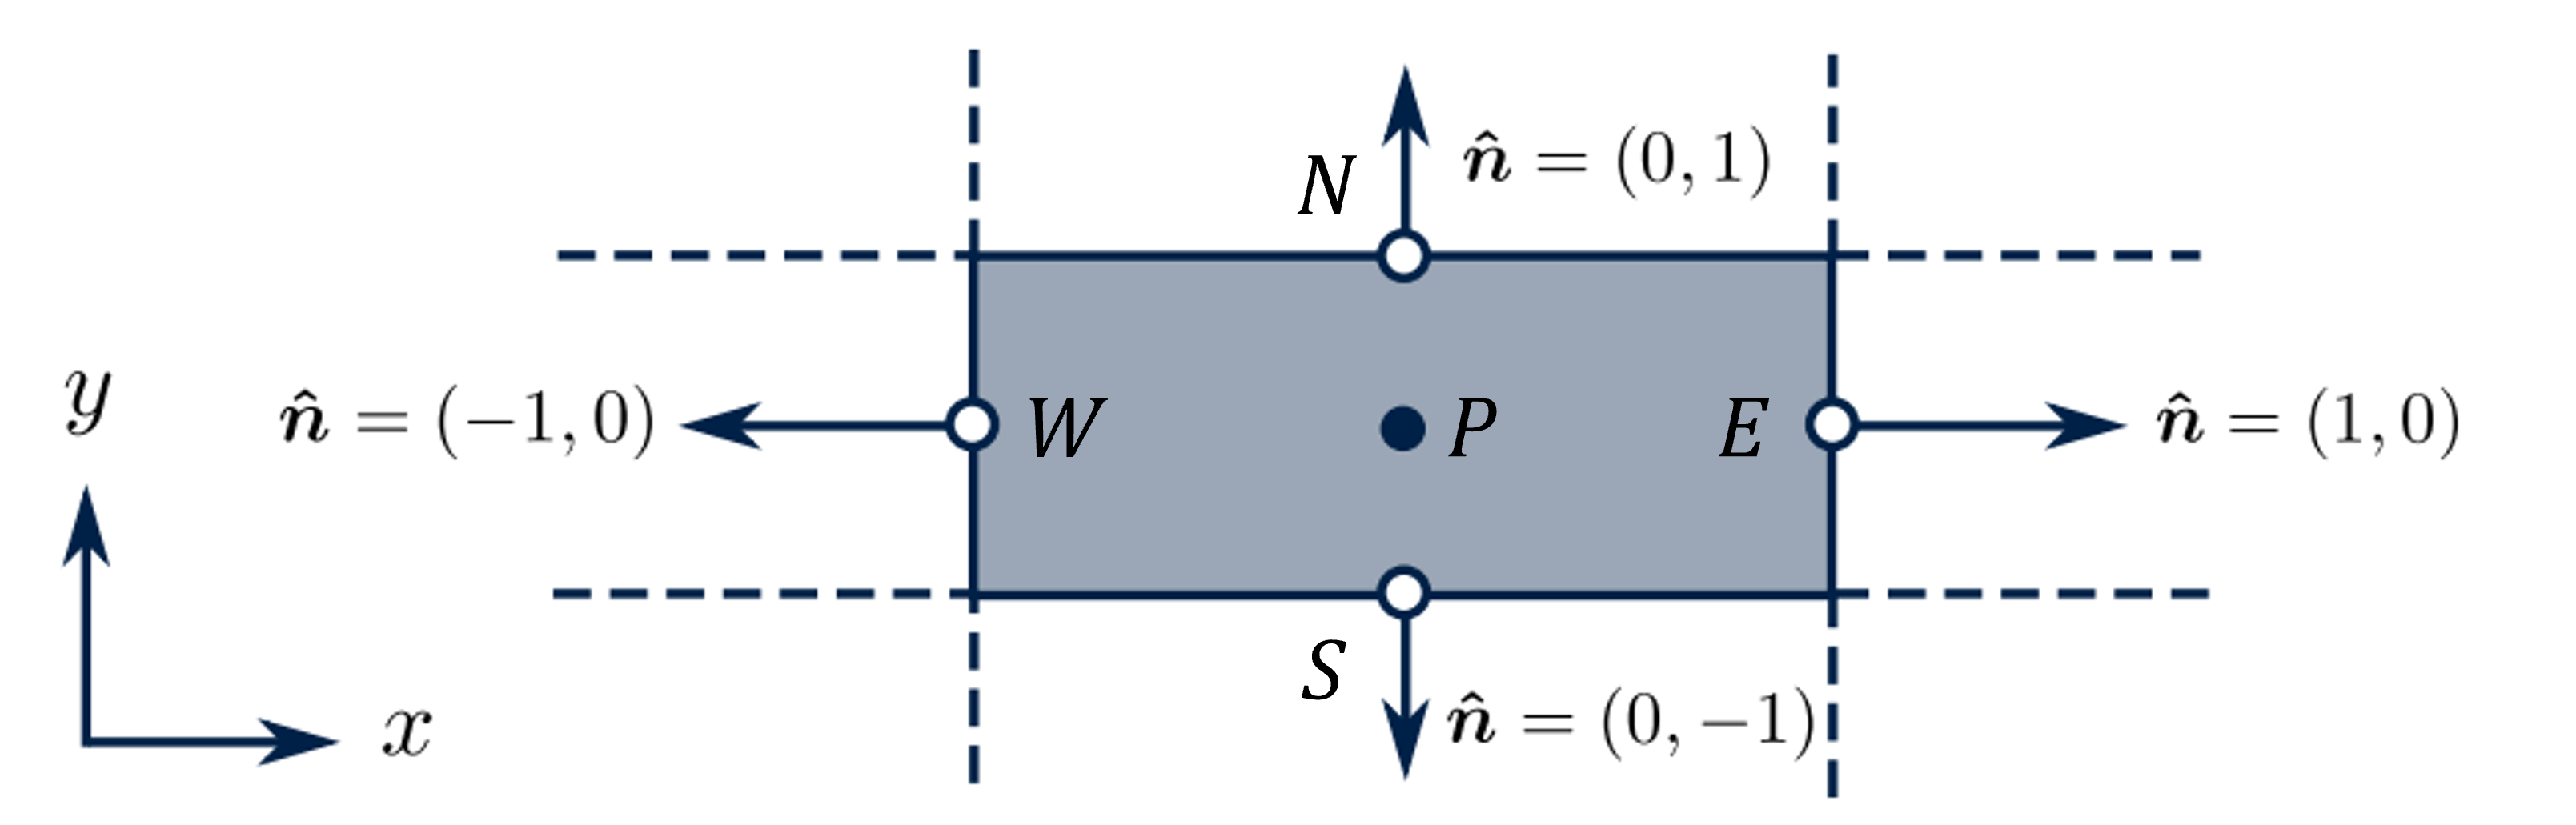
\includegraphics[scale=0.3]{normales_celda.png}
    \caption{ \centering{Vectores normales en direcciones norte ($N$), sur ($S$), este($E$) y oeste ($W$) para una celda 2D}}
    \label{norm_P}
\end{figure}

Teniendo lo anterior en mente y sabiendo que el término difusivo debe ser igual a la suma de los flujos en las fronteras con celdas vecinas ($ \int_S \left[ \Gamma \frac{\partial \phi}{\partial x_j} \hat{n}_j \right] dS = F_N + F_S + F_E + F_W $), pudo usarse el esquema de diferenciación central (CDS) para obtener:

\begin{equation*}
    \begin{split}
    F_e = \Gamma_e \frac{\phi_e-\phi_p}{x_E - x_P} \Delta y \quad ; \quad  F_w = -\Gamma_w \frac{\phi_p-\phi_w}{x_P - x_W} \Delta y \\
    \\[0.1cm]    
    F_n = \Gamma_n \frac{\phi_n-\phi_p}{y_N - y_P} \Delta x \quad ; \quad  F_s = -\Gamma_s \frac{\phi_p-\phi_s}{y_P - y_s} \Delta x        
    \end{split}    
\end{equation*}

La ecuación \eqref{int_S_eq1} fue reescrita de la siguiente manera:

\begin{multline}
    \frac{\Gamma_e \Delta y}{x_E-x_P} \phi_e + \frac{\Gamma_w \Delta y}{x_P-x_W} \phi_w + \frac{\Gamma_n \Delta x}{y_N-y_P} \phi_n \\
    + \frac{\Gamma_s \Delta x}{y_P-y_S} \phi_s - \frac{\Gamma_e \Delta y}{x_E-x_P} \phi_p - \frac{\Gamma_w \Delta y}{x_P-x_W} \phi_p \\
    - \frac{\Gamma_n \Delta x}{y_N-y_P} \phi_p - \frac{\Gamma_s \Delta x}{y_P-y_S} \phi_p + q_{\phi} \Delta x \Delta y  = 0
\end{multline}

Si se agrupa en coeficientes ($a_i$) para cada celda vecina, se reescribe la ecuación de la siguiente manera:

\begin{multline}
    a_E\phi_e + a_W\phi_w + a_N\phi_n + a_S\phi_s - \\
    \underbrace{(a_E+a_W+a_N+a_S)}_{\overset{a_P}{}} \phi_p = -q_{\phi} \Delta x \Delta y 
    \label{dis_int}
\end{multline}

La ecuación \eqref{dis_int} corresponde a la discretización general cuando una celda está rodeada por vecinas en todas las direcciones, es decir que se trata de la discretización para las \textbf{celdas internas}. 

Para las celdas que tienen una o más fronteras en su vecindad, se realizó la discretización correspondiente; a continuación se muestra para cada celda que tiene condiciones de frontera:

Para la \textbf{frontera norte}, en este caso tipo Neumann $(\partial T/\partial y=0)$, el coeficiente $a_N$ no aporta ni en las celdas vecinas ni en el coeficiente $a_P$ y el flujo establecido por la condición de frontera Neumann pasa a contribuir al lado conocido (en este caso es cero).

\begin{multline}
    a_E\phi_e + a_W\phi_w + a_S\phi_s - \underbrace{(a_E+a_W+a_S)}_{\overset{a_{P1}}{}} \phi_p \\ 
    = -q_{\phi} \Delta x \Delta y 
    \label{dis_N}
\end{multline}

En la \textbf{frontera sur} de tipo Dirichlet, el coeficinte $a_S$ no contribuye únicamente en las celdas vecinas pero si contribuye en el lado conocido.

\begin{multline}
    a_E\phi_e + a_W\phi_w + a_N\phi_n - \underbrace{(a_E+a_W+a_N+a_S)}_{\overset{a_{P}}{}} \phi_p \\ 
    = -q_{\phi} \Delta x \Delta y - a_S \phi_s 
    \label{dis_S}
\end{multline}

Para la \textbf{frontera este}, que también es tipo Dirichlet, ocurre algo análogo al caso de la frontera sur pero con el coeficiente $a_E$.

\begin{multline}
    a_W\phi_w + a_N\phi_n + a_S\phi_s - \underbrace{(a_E+a_W+a_N+a_S)}_{\overset{a_{P}}{}} \phi_p \\
    = -q_{\phi} \Delta x \Delta y - a_E \phi_e 
    \label{dis_E}
\end{multline}

Y de igual forma ocurre con la \textbf{frontera oeste} y el coeficiente $a_W$.

\begin{multline}
    a_E\phi_e + a_N\phi_n + a_S\phi_s - \underbrace{(a_E+a_W+a_N+a_S)}_{\overset{a_{P}}{}} \phi_p \\
    = -q_{\phi} \Delta x \Delta y - a_W\phi_w 
    \label{dis_W}
\end{multline}

En las celdas de las esquinas se tienen dos condiciones de frontera simultáneamente, y es por ello que sus efectos se combinan. Para el caso de la \textbf{celda noroeste} se obtuvo:

\begin{multline}
    a_E\phi_e + a_W\phi_w + a_S\phi_s - \underbrace{(a_E+a_W+a_S)}_{\overset{a_{P1}}{}} \phi_p \\
    = -q_{\phi} \Delta x \Delta y - a_W\phi_w
    \label{dis_NW}
\end{multline}

En el caso de la \textbf{celda noreste} se logró:

\begin{multline}
    a_W\phi_w + a_W\phi_w + a_S\phi_s - \underbrace{(a_E+a_W+a_S)}_{\overset{a_{P1}}{}} \phi_p \\
    = -q_{\phi} \Delta x \Delta y - a_E\phi_e
    \label{dis_NE}
\end{multline}

En las dos celdas inferiores hay dos condiciones Dirichlet aplicadas. Para el caso de la \textbf{celda suroeste} se llegó a:

\begin{multline}
    a_E\phi_e + a_N\phi_n - \underbrace{(a_E+a_W+a_N+a_S)}_{\overset{a_{P}}{}} \phi_p \\
    = -q_{\phi} \Delta x \Delta y - a_S\phi_s - a_W\phi_w 
    \label{dis_SW}
\end{multline}

Y finalmente para la \textbf{celda sureste}:

\begin{multline}
    a_W\phi_w + a_N\phi_n - \underbrace{(a_E+a_W+a_N+a_S)}_{\overset{a_{P}}{}} \phi_p \\
    = -q_{\phi} \Delta x \Delta y - a_S\phi_s - a_E\phi_e 
    \label{dis_SE}
\end{multline}

Así pues las ecuaciones \eqref{dis_int} a \eqref{dis_SE} corresponden a las discretizaciones para los nueve tipos de celdas que hay en el dominio computacional (internas, con una y con dos condiciones de frontera).

\section{Problema con solución analítica}
El problema con solución analítica se lleva a cabo en el mismo dominio, pero con condiciones de frontera diferentes, por lo que el código y la discretización cambia ligeramente.

$$
\begin{array}{|cc|}
    \hline \text { Frontera } & \text { Condición } \\
    \hline \text { Norte } & T=150^{\circ} \mathrm{C} \\
    \text { Sur } & T=15^{\circ} \mathrm{C} \\
    \text { Oeste } & T=15^{\circ} \mathrm{C} \\
    \text { Este } & T=15^{\circ} \mathrm{C} \\
    \hline \text { Conduct. } & \kappa=1 \\
    \text { Fuente } & B=0 \\
    \hline
\end{array}
$$

Este problema tiene la solución analítica dada por:

\begin{multline}
    T_{adimensional}(x,y)\\
    =\frac{2}{\pi}\cdot\sum_{n_{impar}}^\infty\frac{sinh(n\pi x/H)}{sinh(n\pi L/H)}\cdot sin(\frac{n\pi y}{H})
    \label{Sol_An_Ad}
\end{multline}

Para darle dimensiones de $^{\circ}\mathrm{C}$ se realizó el siguiente procedimiento:

\begin{equation}
    T(x,y)=(T_{max}-T_{min})\cdot T_{adimensional}(x,y) + T_{min}
    \label{Sol_An}
\end{equation}

\section{Método iterativo Gauss-Seidel}

Se escogió el método iterativo de Gauss-Seidel para la implementación en código ya que es intuitivo y fácil de escribir en código.

El método tiene el siguiente flujo para resolver el sistema matricial $[A][\phi]=[Q]$ con n incógnitas y n ecuaciones:

\begin{itemize}
	\item Hacer una estimación inicial para todas las incógnitas $\phi_{i}^0$.
	\item Resolver la primera ecuación del sistema de ecuaciones para obtener $\phi_{1}^1$.
	\item Resolver la segunda ecuación del sistema de ecuaciones teniendo en cuenta a $\phi_{1}^1$ para llegar a un valor de $\phi_{2}^1$
	\item Resolver la ecuación m-ésima teniendo en cuenta los nuevos valores de las $m-1$ incógnitas anteriores hasta completar las n ecuaciones.
	\item Calcular el residual de la siguiente forma:
	
	\begin{equation}
    	R=\sum^n|q_{\phi} - (a_P\phi_P + \sum_{j}^{vecinos} a_j\phi_j)|
    	\label{Res}
	\end{equation}
	
	\item Normalizar el residual dividiéndolo entre un flujo característico, así
	
	\begin{equation}
    	F=\sum^n|a_P\phi_P|
    	\label{Flujo_C}
	\end{equation}
	
	\item Comparando el residual normalizado con el criterio de convergencia $\epsilon$ se obtiene:
	
	\begin{equation}
    	\frac{R}{F}\leq\epsilon
    	\label{Res_norm}
	\end{equation}
	
	Si esta desigualdad es verdadera no realice más iteraciones pues el método convergió, si es falsa vuelva al segundo item de esta lista ya que el método no ha convergido.
\end{itemize}

Como métodos de salida del algoritmo se tiene:
\begin{itemize}
    \item Que el residual normalizado sea menor al criterio de convergencia.
    \item Que la diferencia entre el residual normalizado de la iteración anterior y el residual normalizado de la iteración actual sea menor que $1\times 10^{-9}$ y mayor que $0$.
    \item Que al haber pasado $1000$ iteraciones y si el residual normalizado de la iteración anterior es menor que el de la iteración actual.
    
Dado que se decidió utilizar los métodos de salida del método anteriormente mencionados no se usó ninguna librería en particular para el mismo.
\end{itemize}

\section{Códigos}
Los dos casos resueltos en este proyecto cuentan con los mismos archivos de código:

\begin{itemize}
	\item Malla.cpp: Este código tiene el dominio computacional y crea la malla sobre la que se va a trabajar con base en el número de celdas en $x$ y $y$ que se desea. También, tiene una función de refinamiento que permite hacer más fina la malla en secciones que el usuario considere que deberían tener más celdas.
	\item Propiedades.cpp: Este archivo recopila la información de la malla y crea el término fuente $B$ y vector de $\kappa$ ya que para el caso de interés esta varía con la posición en dirección $x$.
	\item Frontera\_t0.cpp: En este archivo se recopila la información de la malla y definen las condiciones de frontera de cada caso. Si fuera necesario definir una condición inicial se haría en este archivo.
	\item Procesamiento.cpp: El código de este archivo empieza por definir la función que ensambla una matriz de coeficientes y términos independientes, definir la función del método Gauss-Seidel que barre la malla de izquierda a derecha desde la frontera sur hasta la frontera norte. En el main se recopila la información de todos los archivos anteriores para pasarla por las funciones anteriormente mencionadas. Durante el procesamiento se muestra en la terminal la iteración y el correspondiente residual normalizado.
	\item Posprocesamiento.py: Se recopilan los resultados obtenidos en el archivo de procesamiento (Temperatura y Residual normalizado). En la terminal se muestran los vectores de $x$ y $y$, también la última iteración y su residual normalizado y crea las gráficas de la malla, distribución de temperatura y residual normalizado en escala logarítmica en formato .eps.
\end{itemize}

\section{Resultados}
\subsection{Caso con solución analítica}

\subsection{Caso de interés}

\section{Conclusiones}

\end{document}
